% Circumscribed Parallelepiped
% Author: Axel Pavillet
\documentclass[tikz,border=10pt]{standalone}
%%%<
\usepackage{verbatim}
%%%>
\begin{comment}
:Title: Circumscribed Parallelepiped
:Tags: 3D;Geometry;Mathematics
:Author: Axel Pavillet
:Slug: parallelepiped

This is a drawing of a tetrahedron inscibed in a parallelepiped. 
See the following reference p. 58-63 \S 189 to 202

  @BOOK{altshiller1935modern,
    title     = {Modern pure solid geometry},
    publisher = {The Macmillan company},
    year      = {1935},
    author    = {Altshiller-Court, N.},
    address   = {New York},
    edition   = {first},
    lccn      = {35024297},
    url       = {http://books.google.ca/books?id=DDYGAQAAIAAJ}
  }
\end{comment}
\begin{document}
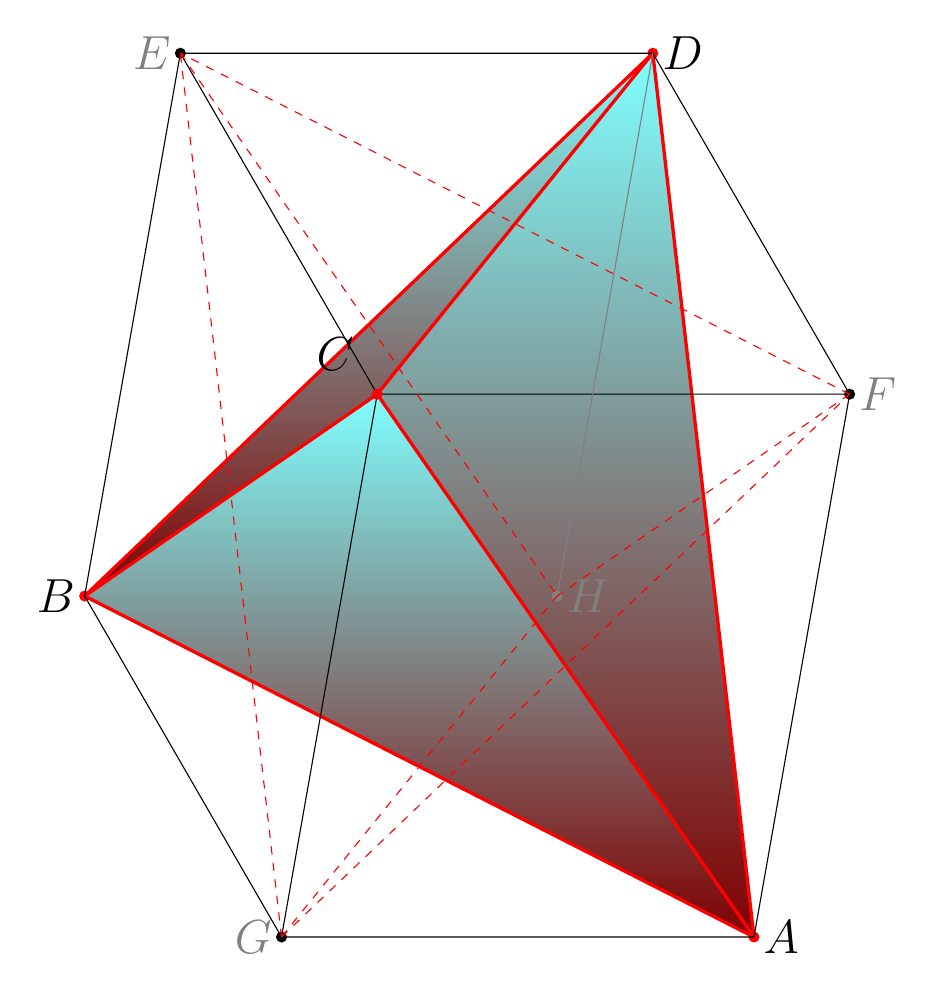
\begin{tikzpicture}[font=\LARGE] 

% Figure parameters (tta and k needs to have the same sign)
% They can be modified at will
\def \tta{ -10.00000000000000 } % Defines the first angle of perspective
\def \k{    -3.00000000000000 } % Factor for second angle of perspective
\def \l{     6.00000000000000 } % Defines the width  of the parallelepiped
\def \d{     5.00000000000000 } % Defines the depth  of the parallelepiped
\def \h{     7.00000000000000 } % Defines the heigth of the parallelepiped

% The vertices A,B,C,D define the reference plan (vertical)
\coordinate (A) at (0,0); 
\coordinate (B) at ({-\h*sin(\tta)},{\h*cos(\tta)}); 
\coordinate (C) at ({-\h*sin(\tta)-\d*sin(\k*\tta)},
                    {\h*cos(\tta)+\d*cos(\k*\tta)}); 
\coordinate (D) at ({-\d*sin(\k*\tta)},{\d*cos(\k*\tta)}); 

% The vertices Ap,Bp,Cp,Dp define a plane translated from the 
% reference plane by the width of the parallelepiped
\coordinate (Ap) at (\l,0); 
\coordinate (Bp) at ({\l-\h*sin(\tta)},{\h*cos(\tta)}); 
\coordinate (Cp) at ({\l-\h*sin(\tta)-\d*sin(\k*\tta)},
                     {\h*cos(\tta)+\d*cos(\k*\tta)}); 
\coordinate (Dp) at ({\l-\d*sin(\k*\tta)},{\d*cos(\k*\tta)}); 

% Marking the vertices of the tetrahedron (red)
% and of the parallelepiped (black)
\fill[black]  (A) circle [radius=2pt]; 
\fill[red]    (B) circle [radius=2pt]; 
\fill[black]  (C) circle [radius=2pt]; 
\fill[red]    (D) circle [radius=2pt]; 
\fill[red]   (Ap) circle [radius=2pt]; 
\fill[black] (Bp) circle [radius=2pt]; 
\fill[red]   (Cp) circle [radius=2pt]; 
\fill[black] (Dp) circle [radius=2pt]; 

% painting first the three visible faces of the tetrahedron
\filldraw[draw=red,bottom color=red!50!black, top color=cyan!50]
  (B) -- (Cp) -- (D);
\filldraw[draw=red,bottom color=red!50!black, top color=cyan!50]
  (B) -- (D)  -- (Ap);
\filldraw[draw=red,bottom color=red!50!black, top color=cyan!50]
  (B) -- (Cp) -- (Ap);

% Draw the edges of the tetrahedron
\draw[red,-,very thick] (Ap) --  (D)
                        (Ap) --  (B)
                        (Ap) -- (Cp)
                        (B)  --  (D)
                        (Cp) --  (D)
                        (B)  -- (Cp);

% Draw the visible edges of the parallelepiped
\draw [-,thin] (B)  --  (A)
               (Ap) -- (Bp)
               (B)  --  (C)
               (D)  --  (C)
               (A)  --  (D)
               (Ap) --  (A)
               (Cp) --  (C)
               (Bp) --  (B)
               (Bp) -- (Cp);

% Draw the hidden edges of the parallelepiped
\draw [gray,-,thin] (Dp) -- (Cp);
                    (Dp) --  (D);
                    (Ap) -- (Dp);

% Name the vertices (the names are not consistent
%  with the node name, but it makes the programming easier)
\draw (Ap) node [right]           {$A$}
      (Bp) node [right, gray]     {$F$}
      (Cp) node [right]           {$D$}
      (C)  node [left,gray]       {$E$}
      (D)  node [left]            {$B$}
      (A)  node [left,gray]       {$G$}
      (B)  node [above left=+5pt] {$C$}
      (Dp) node [right,gray]      {$H$};

% Drawing again vertex $C$, node (B) because it disappeared behind the edges.
% Drawing again vertex $H$, node (Dp) because it disappeared behind the edges.
\fill[red]   (B) circle [radius=2pt]; 
\fill[gray] (Dp) circle [radius=2pt]; 

% From the reference and this example one can easily draw 
% the twin tetrahedron jointly to this one.
% Drawing the edges of the twin tetrahedron
% switching the p_s: A <-> Ap, etc...
\draw[red,-,dashed, thin] (A)  -- (Dp)
                          (A)  -- (Bp)
                          (A)  --  (C)
                          (Bp) -- (Dp)
                          (C)  -- (Dp)
                          (Bp) --  (C);
\end{tikzpicture}
\end{document}
